\documentclass[11pt,a4paper]{article}
\usepackage[T1]{fontenc}
\usepackage{lmodern,microtype,amsmath,amssymb,booktabs,tabularx,array}
\usepackage[margin=21mm,headheight=14pt]{geometry}
\usepackage{xcolor,tikz,hyperref,fancyhdr,enumitem}
\usetikzlibrary{arrows.meta,positioning,calc,fit,backgrounds}
\definecolor{navy}{HTML}{173B52}
\definecolor{teal}{HTML}{087E8B}
\definecolor{pale}{HTML}{EAF5F6}
\definecolor{amber}{HTML}{A75C0A}
\definecolor{warm}{HTML}{FFF3E3}
\definecolor{gray}{HTML}{53616A}
\hypersetup{colorlinks=true,linkcolor=navy,urlcolor=teal,citecolor=teal,
  pdftitle={Learned covariance completion for missing EEG electrodes},
  pdfauthor={AGFL research project}}
\pagestyle{fancy}\fancyhf{}
\fancyhead[L]{\small\color{gray}Learned covariance completion}
\fancyhead[R]{\small\color{gray}Method and verified experiment}
\fancyfoot[C]{\small\thepage}
\renewcommand{\headrulewidth}{0.3pt}
\setlength{\parindent}{0pt}\setlength{\parskip}{5pt}
\setlist[enumerate]{leftmargin=*,itemsep=4pt,topsep=4pt}
\setlist[itemize]{leftmargin=*,itemsep=3pt,topsep=4pt}
\newcolumntype{Y}{>{\raggedright\arraybackslash}X}
\newcommand{\R}{\mathbb R}
\newcommand{\tr}{\operatorname{tr}}
\newcommand{\spplus}{\operatorname{softplus}}
\newcommand{\code}[1]{{\small\nolinkurl{#1}}}
\newcommand{\takeaway}[1]{\par\smallskip\noindent\colorbox{pale}{\parbox{\dimexpr\linewidth-2\fboxsep\relax}{\textbf{Key point.} #1}}\par\smallskip}
\tikzset{box/.style={draw=navy,rounded corners=2pt,fill=white,align=center,
  font=\small,minimum height=12mm,inner sep=5pt},
  learned/.style={box,draw=teal,fill=pale},
  fixed/.style={box,fill=black!3},
  flow/.style={-{Latex[length=2mm]},thick,draw=navy},
  grad/.style={-{Latex[length=2mm]},thick,dashed,draw=amber}}
\begin{document}
\thispagestyle{empty}
{\Huge\bfseries\color{navy} Learned covariance}\par\vspace{3pt}
{\LARGE\color{navy} Completion for missing EEG electrodes}\par\vspace{8pt}
{\large A mathematical and implementation guide}\par\vspace{4pt}
5 October 2026\quad\textbullet\quad Verified CUDA study, version 2

\section{What the method does}
When an electrode is unavailable, its signal is estimated from the electrodes
that remain. A single learned matrix encodes relationships between all 22
channels. The observed subset selects a small linear system; solving it gives
the weights used to fill the missing channels. Observed samples are copied
unchanged. The completed signal is then classified by an already trained,
frozen EEGNet--Transformer.

The trainable component has only \textbf{253 scalar parameters}, describing a
symmetric positive-definite $22\times22$ matrix. It is initialized from training
signals and adjusted using classification, reconstruction and anchoring losses.
There is one fitted matrix per participant and split/training seed, shared across
that task's trials, windows and time samples. It is not recomputed from each
evaluation trial, and it is not a Tucker or low-rank tensor decomposition.

\begin{center}
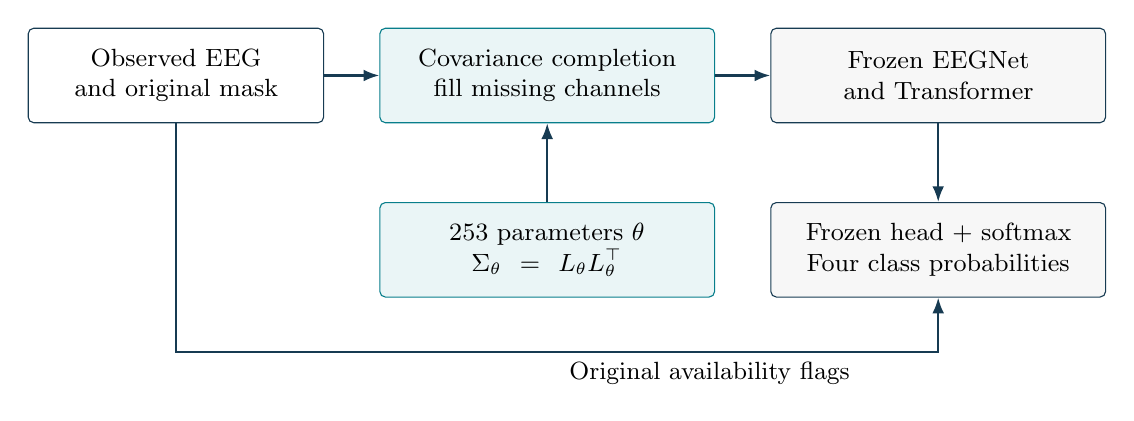
\begin{tikzpicture}[node distance=7mm]
\node[box,text width=34mm] (obs) {Observed EEG\\and original mask};
\node[learned,text width=39mm,right=of obs] (fill) {Covariance completion\\fill missing channels};
\node[fixed,text width=39mm,right=of fill] (net) {Frozen EEGNet\\and Transformer};
\draw[flow] (obs)--(fill);\draw[flow] (fill)--(net);
\node[learned,text width=39mm,below=10mm of fill] (sigma) {253 parameters $\theta$\\$\Sigma_\theta=L_\theta L_\theta^\top$};
\draw[flow] (sigma)--(fill);
\node[fixed,text width=39mm,below=10mm of net] (pred) {Frozen head + softmax\\Four class probabilities};
\draw[flow] (net)--(pred);
\draw[flow] (obs.south)--++(0,-29mm)-|node[pos=.35,below,font=\small]{Original availability flags} (pred.south);
\end{tikzpicture}
\end{center}
{\small The mask also enters the frozen classifier head; predicted samples do not
become ``observed.'' Teal marks the trainable completion component.}

\subsection*{Notation used throughout}
\begin{tabularx}{\linewidth}{@{}lY@{}}\toprule
Symbol & Meaning and dimensions \\ \midrule
$B,C,P,T$ & Batch size; $C=22$ channels; $P=4$ windows; $T=250$ samples/window. \\
$X,M$ & Normalized EEG $X\in\R^{B\times C\times P\times T}$ and Boolean availability $M\in\{0,1\}^{B\times C\times P}$. \\
$O,H$ & Observed and hidden channel indices in one trial/window; $H=\{1,\ldots,C\}\setminus O$, $|O|\geq1$. \\
$\widetilde X$ & Completed EEG with the same shape as $X$. \\
$\theta,\phi$ & Trainable completion parameters and frozen classifier parameters. \\ \bottomrule
\end{tabularx}
\takeaway{The model learns how to fill gaps in the classifier's input. It does
not retrain the classifier or modify the samples that were actually observed.}

\newpage
\section{From training signals to a valid matrix}
\subsection{Normalization and initialization}
Each four-second trial contains 22 EEG channels sampled at 250 Hz, arranged
as four one-second windows. The inherited preprocessing uses 2--30 Hz filtering
within each channel/window. Let $R$ denote these filtered signals. For each
channel $c$, compute the mean $\mu_c$ and population standard deviation $s_c$
using \emph{training trials and all their time samples only}. Then
\begin{equation}
 X_{bcpt}=\frac{R_{bcpt}-\mu_c}{\max(s_c,10^{-8})}.
 \label{eq:norm}
\end{equation}
The same constants are used for validation and later inference. This removes a
training channel mean, not a separate mean for every trial or window.

Collect all $n=N_{\rm train}PT$ training-time channel vectors into
$Q\in\R^{n\times C}$. Initialize from the uncentered second moment of the
already normalized data:
\begin{equation}
 S=\frac1n Q^\top Q,\qquad
 \Sigma_0=\tfrac12(S+S^\top)+\varepsilon I_C,\qquad \varepsilon=10^{-6}.
 \label{eq:init}
\end{equation}
Training centering makes $S$ approximately the population covariance, up to
finite precision. There is no extra per-trial centering or $n-1$ correction.
The diagonal jitter $\varepsilon$ permits a stable Cholesky initialization.
It is distinct from the solve regularization introduced on the next page.

\subsection{Positive definiteness by construction}
A general symmetric matrix can become indefinite during optimization. Instead,
store a vector $\theta\in\R^{C(C+1)/2}=\R^{253}$ containing the free lower-triangle
entries. Define
\begin{equation}
 (L_\theta)_{ij}=
 \begin{cases}
  \theta_{ij}, & i>j,\\
  \spplus(\theta_{ii})+\delta, & i=j,\\
  0, & i<j,
 \end{cases}
 \qquad \Sigma_\theta=L_\theta L_\theta^\top,\quad\delta=10^{-6},
 \label{eq:spd}
\end{equation}
where $\spplus(z)=\log(1+e^z)$, evaluated with a numerically stable routine.
The positive diagonal makes $L_\theta$ invertible. Therefore, for every nonzero $v$,
\begin{equation}
 v^\top\Sigma_\theta v=\|L_\theta^\top v\|_2^2>0.
\end{equation}
This is a full-rank matrix factorization, not a dimensionality reduction.
No orthogonality, unit-column projection or unit-diagonal constraint is applied.

To match the initial covariance, compute $L_0=\operatorname{chol}(\Sigma_0)$.
Copy its off-diagonal entries and initialize its diagonal free parameters by
\begin{equation}
 z_i=(L_0)_{ii}-\delta,\qquad
 (\theta_0)_{ii}=z_i+\log(1-e^{-z_i}).
 \label{eq:inverse}
\end{equation}
Here $z_i>0$ is checked. The expression is the inverse softplus, evaluated
stably in code. Thus both covariance arms start with the same $\Sigma_0$ up
to floating-point precision. The frozen arm retains $\theta_0$; the learned
arm optimizes $\theta$ and keeps a separate, immutable copy of $\theta_0$.

\takeaway{Only the training set determines initialization. Positive definiteness
is maintained structurally, while the matrix's entries can adapt to the task.}

\newpage
\section{Completing one partially observed window}
For one trial/window, write $X_O\in\R^{o\times T}$ for its observed rows,
where $o=|O|$, and let $h=|H|$. Original channel identities determine the rows
and columns extracted from $\Sigma=\Sigma_\theta$; channel order is never lost.

\begin{center}
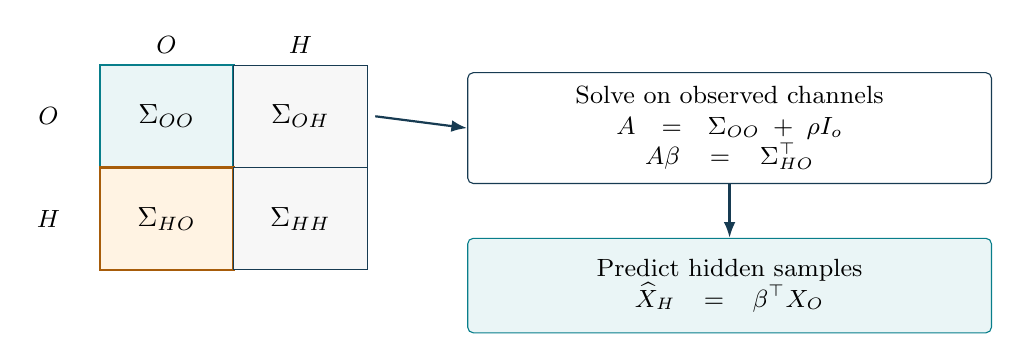
\begin{tikzpicture}
\node[font=\small] at (-.65,1.15) {$O$};\node[font=\small] at (-.65,-.15) {$H$};
\node[font=\small] at (.85,2.05) {$O$};\node[font=\small] at (2.55,2.05) {$H$};
\draw[fill=pale,draw=teal,thick] (0,.5) rectangle (1.7,1.8);
\draw[fill=black!3,draw=navy] (1.7,.5) rectangle (3.4,1.8);
\draw[fill=warm,draw=amber,thick] (0,-.8) rectangle (1.7,.5);
\draw[fill=black!3,draw=navy] (1.7,-.8) rectangle (3.4,.5);
\node at (.85,1.15) {$\Sigma_{OO}$};\node at (2.55,1.15) {$\Sigma_{OH}$};
\node at (.85,-.15) {$\Sigma_{HO}$};\node at (2.55,-.15) {$\Sigma_{HH}$};
\node[box,text width=63mm] (solve) at (8,1) {Solve on observed channels\\$A=\Sigma_{OO}+\rho I_o$\\$A\beta=\Sigma_{HO}^{\top}$};
\node[learned,text width=63mm] (fill) at (8,-1) {Predict hidden samples\\$\widehat X_H=\beta^\top X_O$};
\draw[flow] (3.5,1.15)--(solve.west);\draw[flow] (solve)--(fill);
\end{tikzpicture}
\end{center}
{\small Conceptual block permutation for explanation only. The implementation
indexes the original channel coordinates and restores predictions to those coordinates.}

\subsection{The regularized conditional predictor}
Set a scale-adaptive ridge coefficient using the \emph{whole} matrix:
\begin{equation}
 \rho(\Sigma)=\alpha\frac{\tr(\Sigma)}{C},\qquad\alpha=10^{-3}.
 \label{eq:rho}
\end{equation}
The missing-channel estimate is
\begin{equation}
 \boxed{\widehat X_H=\Sigma_{HO}(\Sigma_{OO}+\rho I_o)^{-1}X_O.}
 \label{eq:completion}
\end{equation}
Here $\Sigma_{HO}$ has shape $h\times o$. Code does not form an inverse:
it solves $A\beta=\Sigma_{HO}^{\top}$ with $\beta\in\R^{o\times h}$ and
multiplies $\beta^\top X_O$. One solve supplies the weights for all 250 time
samples, and trial/windows with identical masks are grouped.

For nonzero $u\in\R^o$, $u^\top Au=u^\top\Sigma_{OO}u+\rho\|u\|^2>0$.
The system consequently has a unique solution in exact arithmetic. Covariance
construction and solves use float64, with finite-value checks; the predictions
are cast back to the signal dtype. Positive definiteness alone does not promise
perfect numerical conditioning for arbitrary parameters.

\subsection{Why this expression is reasonable}
Under a zero-mean Gaussian model, the conditional mean of hidden coordinates
is $\Sigma_{HO}\Sigma_{OO}^{-1}x_O$ \cite{gpml}. Adding independent observation
noise with variance $\rho$ gives Equation~\eqref{eq:completion}. This is a
motivation for the regularized predictor, not an assertion that actual EEG is
Gaussian or that its noise variance was estimated. The implementation retains
the observed values exactly, rather than denoising them under that model.

Finally, fill only hidden entries:
\begin{equation}
 \widetilde X_{c,t}=\begin{cases}X_{c,t},&c\in O,\\
 \widehat X_{c,t},&c\in H.\end{cases}
 \label{eq:copy}
\end{equation}
An all-observed window needs no prediction. An all-missing window is rejected:
this method requires at least one observed electrode.

\newpage
\section{A worked example and useful properties}
\subsection{Three channels, one missing}
Consider the illustrative positive-definite matrix
\begin{equation}
 \Sigma=\begin{pmatrix}1&0.6&0.2\\0.6&1&0.4\\0.2&0.4&1\end{pmatrix},
 \qquad x_O=\begin{pmatrix}1\\-0.5\end{pmatrix},\quad O=\{1,3\},\ H=\{2\}.
\end{equation}
The trace rule gives $\rho=0.001$. Therefore
\begin{align}
 A&=\begin{pmatrix}1.001&0.2\\0.2&1.001\end{pmatrix},&
 \Sigma_{HO}&=\begin{pmatrix}0.6&0.4\end{pmatrix},\\
 \beta&=A^{-1}\begin{pmatrix}0.6\\0.4\end{pmatrix}
       \simeq\begin{pmatrix}0.541164\\0.291476\end{pmatrix},&
 \widehat x_2&=0.541164(1)+0.291476(-0.5)\simeq0.395426.
\end{align}
The completed vector is $(1,\,0.395426,\,-0.5)^\top$. The first and third
samples are copied, not re-estimated. This toy calculation is not a measured
EEG result; it shows the arithmetic used at each time sample.

\begin{center}
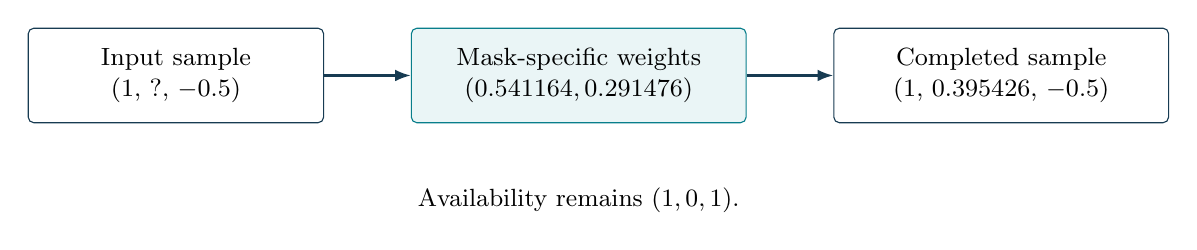
\begin{tikzpicture}[node distance=11mm]
\node[box,text width=34mm] (in) {Input sample\\$(1,\,?,\,-0.5)$};
\node[learned,text width=39mm,right=of in] (mix) {Mask-specific weights\\$(0.541164,0.291476)$};
\node[box,text width=39mm,right=of mix] (out) {Completed sample\\$(1,\,0.395426,\,-0.5)$};
\draw[flow] (in)--(mix);\draw[flow] (mix)--(out);
\node[font=\small,below=7mm of mix] {Availability remains $(1,0,1)$.};
\end{tikzpicture}
\end{center}

\subsection{What is shared and what changes}
\begin{tabularx}{\linewidth}{@{}lY@{}}\toprule
Quantity & Dependence \\ \midrule
$\Sigma_\theta$ & Shared over every trial, window and sample in one fitted task. \\
$O,H$ & Determined by the known electrode mask for each trial/window. \\
$W_{H\leftarrow O}=\beta^\top$ & Depends on the mask and $\Sigma_\theta$, but not on signal amplitudes. \\
$\widehat X_H$ & Depends linearly on the observed signal through $W_{H\leftarrow O}X_O$. \\ \bottomrule
\end{tabularx}

For a fixed mask, this is an instantaneous spatial linear predictor. It mixes
electrodes at the same sample time, independently within each window. It does
not learn a temporal filter or use another window to infer the missing signal.
The downstream EEGNet--Transformer still models time and can mix windows.

The weights need not be positive and need not sum to one. Thus this is neither
a convex average nor distance-based interpolation. One shared SPD matrix
couples the predictors for all masks; they are not independently trained
regression heads for every possible subset.

The prediction weights are invariant to a positive global scale of $\Sigma$:
\begin{equation}
 W_{H\leftarrow O}(a\Sigma)
 =a\Sigma_{HO}\bigl(a\Sigma_{OO}+a\rho(\Sigma)I_o\bigr)^{-1}
 =W_{H\leftarrow O}(\Sigma),\quad a>0.
\end{equation}
This follows specifically from the trace-scaled ridge. The parameter anchor
still depends on scale through $\theta$, so the entire training objective is
not scale-invariant.

\takeaway{The learned object is a compact, shared family of mask-dependent
linear completion rules. Its usefulness must be judged by held-out prediction,
not by treating matrix entries as physiological connectivity.}

\newpage
\section{Connecting completion to a frozen classifier}
\subsection{Forward route and availability flags}
Let $g_\phi$ denote the historical EEGNet--Transformer computation applied to
\emph{completed} signals, with original mask flags appended at the output head.
The adapted predictor is
\begin{equation}
 p_\theta(y\mid X_O,M)=\operatorname{softmax}
   \bigl(g_\phi(\widetilde X_\theta,M)\bigr),\qquad\phi\ \text{fixed}.
\end{equation}
The historical backbone uses an EEGNet front end, inspired by the compact EEG
architecture of Lawhern et al.\ \cite{eegnet}, followed by a temporal Transformer.
The exact local route is shown below.

\begin{center}
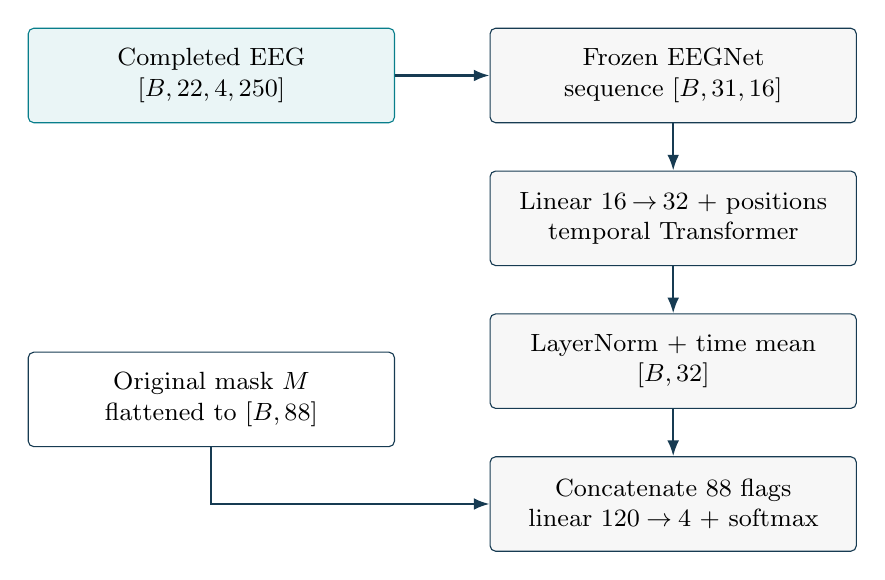
\begin{tikzpicture}[node distance=6mm]
\node[learned,text width=43mm] (fill) {Completed EEG\\$[B,22,4,250]$};
\node[fixed,text width=43mm,right=12mm of fill] (eeg) {Frozen EEGNet\\sequence $[B,31,16]$};
\node[fixed,text width=43mm,below=of eeg] (tf) {Linear $16\!\to\!32$ + positions\\temporal Transformer};
\node[fixed,text width=43mm,below=of tf] (pool) {LayerNorm + time mean\\$[B,32]$};
\node[fixed,text width=43mm,below=of pool] (head) {Concatenate 88 flags\\linear $120\!\to\!4$ + softmax};
\draw[flow] (fill)--(eeg);\draw[flow] (eeg)--(tf);
\draw[flow] (tf)--(pool);\draw[flow] (pool)--(head);
\node[box,text width=43mm,below=29mm of fill] (mask) {Original mask $M$\\flattened to $[B,88]$};
\draw[flow] (mask.south)|-(head.west);
\end{tikzpicture}
\end{center}
The Transformer has one pre-normalized layer, four heads, feed-forward width
64, GELU and fixed sinusoidal positions. The EEGNet front end concatenates the
four windows into 1,000 samples for its inherited convolutions; only completion
and preprocessing are window-local. All backbone weights and BatchNorm statistics
remain fixed, and dropout remains disabled.

\textbf{Do not mask the completed signal back to zero.} The adapter feeds filled
values directly into the existing layers. It retains $M$ for the 88 head features.
Calling an ordinary raw-masking backbone route on $(\widetilde X,M)$ would erase
the completion. Entirely full-input batches bypass the completer and call the
original model exactly, preserving full-input predictions across strategies.

\subsection{A frozen network still transmits input gradients}
Freezing $\phi$ means not updating it; it does not mean wrapping its training
forward pass in a no-gradient context. Classification derivatives must reach
$\widetilde X_\theta$ and then $\theta$. To see the solve derivative, equivalently
write $AZ=X_O$, $\widehat X_H=\Sigma_{HO}Z$. For fixed observed input,
\begin{align}
 dZ&=-A^{-1}(dA)Z, & dA&=d\Sigma_{OO}+d\rho\,I_o,\\
 d\widehat X_H&=(d\Sigma_{HO})Z-\Sigma_{HO}A^{-1}(dA)Z,
 & d\rho&=\frac{\alpha}{C}\tr(d\Sigma).
\end{align}
Autograd differentiates the solve and the Cholesky parameterization, including
the dependence of $\rho$ on the learned diagonal. No eigendecomposition or
explicit inverse is differentiated.

\newpage
\section{Learning objective and optimization}
Training starts with complete training trials. Artificial masks hide some
electrodes from the forward computation, while their true samples remain
available only as reconstruction targets. For a batch of size $B$, labels
$y_b\in\{0,1,2,3\}$, and scalar hidden-sample index set
$\mathcal H=\{(b,c,p,t):M_{bcp}=0\}$, define
\begin{align}
 \mathcal L_{\rm cls}
  &=-\frac1B\sum_{b=1}^B\log p_\theta(y_b\mid X_{b,O},M_b),\\
 \mathcal L_{\rm rec}
  &=\frac{\sum_{(b,c,p,t)\in\mathcal H}
       (\widetilde X_{bcpt}-X_{bcpt})^2}{\max(1,|\mathcal H|)},\\
 \mathcal L_{\rm anchor}
  &=\frac1{253}\|\theta-\theta_0\|_2^2,\\
 \boxed{\mathcal L
  =\mathcal L_{\rm cls}+0.1\mathcal L_{\rm rec}
    +10^{-4}\mathcal L_{\rm anchor}.}
 \label{eq:loss}
\end{align}
The reconstruction denominator counts hidden scalar samples over the entire
batch. Observed entries do not enter that error. The anchor is on the free
Cholesky parameters, not on $\Sigma$ itself. It discourages large departures
from the training-statistics initialization. No Gaussian likelihood is optimized.

\begin{center}
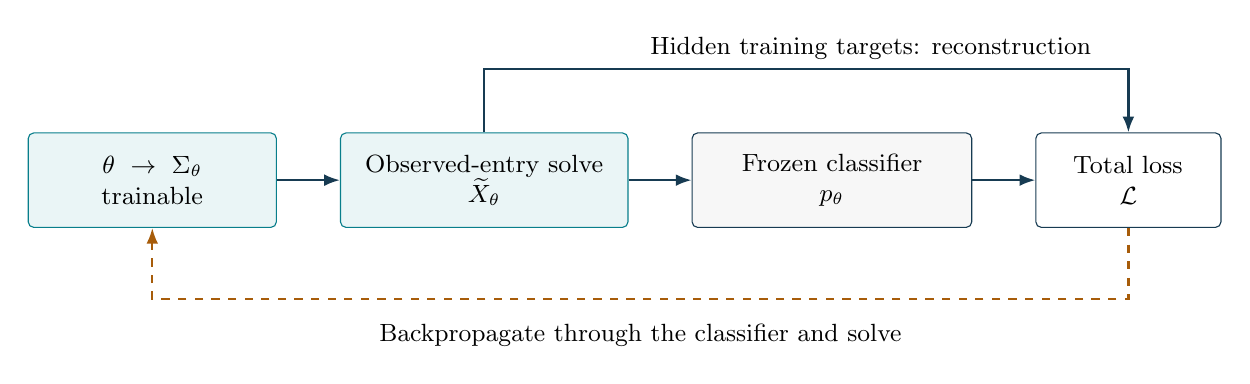
\begin{tikzpicture}[node distance=8mm]
\node[learned,text width=28mm] (theta) {$\theta\to\Sigma_\theta$\\trainable};
\node[learned,text width=33mm,right=of theta] (fill) {Observed-entry solve\\$\widetilde X_\theta$};
\node[fixed,text width=32mm,right=of fill] (net) {Frozen classifier\\$p_\theta$};
\node[box,text width=20mm,right=of net] (loss) {Total loss\\$\mathcal L$};
\draw[flow] (theta)--(fill);\draw[flow] (fill)--(net);\draw[flow] (net)--(loss);
\draw[flow] (fill.north)--++(0,8mm)-|node[pos=.3,above,font=\small]{Hidden training targets: reconstruction} (loss.north);
\draw[grad] (loss.south)--++(0,-9mm)-| (theta.south);
\node[font=\small,anchor=north] at ($(theta.south)!0.5!(loss.south)+(0,-11mm)$)
  {Backpropagate through the classifier and solve};
\end{tikzpicture}
\end{center}

\subsection*{One training run}
\begin{enumerate}
\item Load the historical participant/seed split and frozen classifier. Verify
its original full-input predictions. Fit normalization and $\Sigma_0$ on training data.
\item At each epoch, draw paired per-trial masks: retain 22, 16 or 6 electrodes
with equal probability. For nonfull input, static/dynamic random loss is equally
likely. Preserve channel identities and partition-disjoint mask subsets.
\item Compute Equation~\eqref{eq:loss}, backpropagate only to $\theta$, clip its
gradient norm at 1, and take an Adam step. Keep the backbone in evaluation mode.
Wholly full batches skip the optimizer step, including any anchor-only update.
\item Evaluate the fixed degraded validation bank. Retain the best checkpoint;
restore its numeric parameters after training. No test targets enter this loop.
\end{enumerate}
\begin{tabularx}{\linewidth}{@{}lY@{}}\toprule
Optimizer & Adam; learning rate $10^{-3}$; batch size 32; zero weight decay. \\
Budget & At most 100 epochs; at least 10 before stopping; patience 20. \\
Selection & Highest mean degraded validation balanced accuracy; ties: lower
log loss, then earlier epoch. Epoch zero is eligible. \\
Additional settings & No scheduler, no mixed precision; only completion parameters update. \\ \bottomrule
\end{tabularx}

\newpage
\section{What the completed experiment shows}
\subsection{Paired validation protocol}
The study uses nine BCI IV 2a participants, T-session data, and seeds 0, 1 and 2.
Each seed defines a participant-specific, approximately 60/20/20 train/validation/test
split inherited from the earlier study; this screen uses training and validation
only. Seeds vary splits as well as training randomness. There are 27 tasks and
54 supervised fits: learned covariance and learned Tucker in each task. Zero,
frozen covariance and frozen Tucker are paired controls; no backbone is retrained.

Evaluate all 22 electrodes once, plus static and dynamic random retention of
16 and 6 electrodes, each with five paired mask repeats. Static masks retain
one subset across all windows. The implemented dynamic schedule uses subsets
$A,B,A,A$ over the four windows, with $A\ne B$ and equal retained counts.
Completion selection and reported degraded evaluation use the same masks.

For each cell, balanced accuracy is the average of the four class recalls:
\begin{equation}
 \mathrm{BA}=\frac14\sum_{k=0}^3
 \frac{\sum_b\mathbf 1[y_b=k,\ \arg\max_j p_{bj}=k]}{\sum_b\mathbf 1[y_b=k]}.
\end{equation}
Average mask repeats, then seeds within a participant, then participants equally.
The overall degraded score also averages the four degraded conditions equally.
The 16- and 6-electrode columns below each average static and dynamic conditions.

\subsection{Verified cohort results}
\begin{center}
\begin{tabular}{@{}lrrrr@{}}\toprule
Completion & Overall BA & 16 retained & 6 retained & Log loss\\
 & (\%) & BA (\%) & BA (\%) & overall\\ \midrule
Zero filling & 34.17 & 36.68 & 31.66 & 2.317\\
Frozen Tucker & 36.01 & 40.12 & 31.91 & 2.178\\
Learned Tucker & 38.45 & 41.87 & 35.04 & 2.049\\
Frozen covariance & 49.57 & 58.27 & 40.87 & 1.465\\
\textbf{Learned covariance} & \textbf{55.92} & \textbf{59.81} & \textbf{52.04} & \textbf{1.149}\\ \bottomrule
\end{tabular}
\end{center}
Log loss uses natural logarithms and lower is better. All strategies have
identical full-input predictions: cohort balanced accuracy is 64.87\%.
Completion has no full-input accuracy-gain objective.

Learned covariance improves on frozen covariance by \textbf{6.35 percentage
points}, with positive participant averages in 9/9 participants. The exploratory
95\% participant-bootstrap interval is $[4.01,9.45]$ points (2,000 resamples,
seed 20261005). The gain is 1.54 points with 16 electrodes and 11.17 points
with 6 electrodes. These condition gains are descriptive, not separate
confirmatory hypothesis tests.

Learned Tucker gains 2.44 points over frozen Tucker, meeting the declared
primary exploratory screen ($\geq2$ points and $\geq6/9$ positive participants).
Nevertheless, learned covariance exceeds learned Tucker by 17.47 points.
Covariance comparisons are secondary contrasts in the original declaration;
the primary endpoint has not been changed retrospectively.

\takeaway{This screen favors learned covariance as the candidate for an
independent follow-up. It supports a practical choice within this tested
pipeline, not a universal claim about covariance versus tensor models.}

\newpage
\section{Interpretation, safeguards and reproduction}
\subsection{What the evidence can and cannot establish}
After supervised updates, $\Sigma_\theta$ parameterizes useful completion rules.
It is not a calibrated physiological covariance or causal connectivity estimate.
The model supplies point predictions, without validated uncertainty estimates.

Both backbone and completion checkpoints used validation selection. Epoch zero
reproduces the frozen initialization and is eligible, so the selected model
cannot have a lower \emph{selection score} than that initialization. Nonnegative
gains on this bank are partly built into selection. Bootstrap intervals do not
correct selection optimism, validation reuse or multiple comparisons.
Independent evaluation with settings frozen is still required.

Simulated missingness on complete trials does not establish robustness to corrupt
observed channels, missing calibration channels, unseen participants or new
sessions. Why Tucker underperforms is unresolved; different ranks, losses or
backbones require new experiments.

\subsection{Implementation safeguards}
\begin{itemize}
\item Select hidden NaN/Inf values away with \code{torch.where} before arithmetic;
zero multiplication cannot safely remove NaNs. Reject observed nonfinite samples
and all-missing windows. Preserve observed samples and original mask flags.
\item Calibration stays on CPU; optimization and prediction use CUDA. The
verified execution disables TF32, autocast and fused MHA fastpath, with
deterministic algorithms. CPU/GPU full-input tolerance is
$\mathrm{rtol}=10^{-4}$, $\mathrm{atol}=10^{-6}$; same-device saved-state replay is exact.
\end{itemize}

\subsection{Source and evidence map}
\begin{tabularx}{\linewidth}{@{}lY@{}}\toprule
Definition & Local source or artifact \\ \midrule
Covariance and masking & \code{inm/task_driven_completion/completion.py} \\
Differentiable backbone adapter & \code{inm/task_driven_completion/adapters.py} \\
CUDA training and audit & \code{inm/task_driven_completion_cuda/} \\
Frozen declaration & \code{configs/task-driven-completion-cuda-v2.json} \\
Measured tables and provenance & \code{results/task-driven-completion-cuda-v2/report/} \\
Independent completion review & \code{.session-runs/task-driven-completion-cuda/completion-verification/verification.json} \\ \bottomrule
\end{tabularx}
All 27 tasks / 54 supervised fits completed. Independent GPU audits exactly
replayed 2,835 cells; a subsequent review verified hashes and recomputed metrics,
aggregation and intervals. Study identity:\par
{\footnotesize\nolinkurl{74bfeb36445f3b0d365fac8ca03514e9e8e359c2c205b277e0389bf2922eb071}}

Build: {\small\verb|make -C docs/concept learned_covariance.pdf|}.
Diagrams are editable TikZ vectors; no external images are needed.

\begin{thebibliography}{2}\small
\bibitem{gpml} C. E. Rasmussen and C. K. I. Williams.
\emph{Gaussian Processes for Machine Learning}. MIT Press, 2006, Appendix A.2.
\href{https://gaussianprocess.org/gpml/chapters/RWA.pdf}{Gaussian conditioning and matrix identities}.
\bibitem{eegnet} V. J. Lawhern et al.
\emph{EEGNet: A Compact Convolutional Network for EEG-based Brain--Computer Interfaces}.
\href{https://arxiv.org/abs/1611.08024}{arXiv:1611.08024}.
\end{thebibliography}
\end{document}
